\section{\LARGE{Elettroforesi SDS-PAGE}}

\vspace{0.6cm}


\subsection{Sommario}

\subsubsection{Scopo}

Lo scopo di questa esperienza e' effettuare
l'elettroforesi
delle proteine estratte nell'esperienza 10 tramite la
tecnica SDS-PAGE

\subsubsection{Cenni teorici}

Solitamente l'elettroforesi ha la capacit\`a di separare le proteine secondo sia
la carica che la massa.
L'elettroforesi SDS-PAGE, che si effettua in gel di acrilammide, si differenzia
rispetto ad altre procedure in quanto la separazione delle proteine
avviene solo in base al solo peso molecolare, indipendentemente dalla carica.
Ci\`o \`e possibile grazie alla propriet\`a denaturante dell'SDS,
che permette di mantenere costante il rapporto massa-carica per ogni proteina denaturata.
L'SDS, acronimo di Laurilsolfato di sodio, e' un tensioattivo in grado di denaturare le proteine e
caricarle negativamente in modo proporzionale alla loro massa.

Il gel e' diviso in due parti, stacking gel e running gel. Lo stacking gel
ha lo scopo di allineare le proteine, portandole tutte allo stesso livello e per
questo contiene una percentuale minore di acrilammide.
Il running gel ha invece il compito di permettere alle proteine di separarsi a
seconda della carica.

\subsubsection{Strumenti e materiali utilizzati}

\begin{itemize}
\item Guanti in lattice
\item Provette Eppendorf (2ml)
\item Micropipette (100-1000 e 2-200 ml)
\item Falcon (50mL)
\item Carta bibula
\item Apparato per casting del gel elettroforetico
\end{itemize}

\subsubsection{Soluzioni e composti}

\begin{itemize}
\item Laemmli Sample Buffer 4X
\item Acrilammide/bis
\item 1,5M Tris-HCl, pH 8,8
\item Tris base
\item Glicina
\item 10\% soluzione SDS
\item 10\% ammonio persolfato
\item TEMED
\item isopropanolo
\item ddH20
\item Proteine da analizzare 20ug (estratte nell'esperienza 10)
\item Tris base
\item Glicina
\item 10\% soluzione SDS
\end{itemize}


\subsection{Procedimento}

\subsubsection{Preparazione del Running/Resolving gel}

\begin{enumerate}
	\item Predisporre l'apparato necessario al casting del gel elettroforetico.

	\item Miscelare tutti i componenti della tabella 1 in una Falcon da 50mL.

	\item Distribuire velocemente la miscela tra i vetri dell'apparato, e' importante
	tenere l'eccesso del gel all'interno della Falcon, per stabilire quando il gel
	si sara' solidificato.

	\item Stratificare sino a riempimento con alcol isopropilico.
	Questa fase e' necessaria per limitare il contatto con l'aria
	del gel che si sta solidificando e contemporaneamente	permettere
	un livellamento del gel grazie al peso dell'alcol.
	\`E importante notare che in questa fase l'alcol e
	il gel non si mescolano.

	\item Attendere la polimerizzazione (confermata dalla quantit\`a di
	gel lasciata nella Falcon)
\end{enumerate}

\subsubsection{Preparazione dell'Electrode Running Buffer 10X}

\subsubsection{Preparazione dello stacking gel}

% \begin{enumerate}


	% \begin{figure}[H]
	% 	\centering
	% 	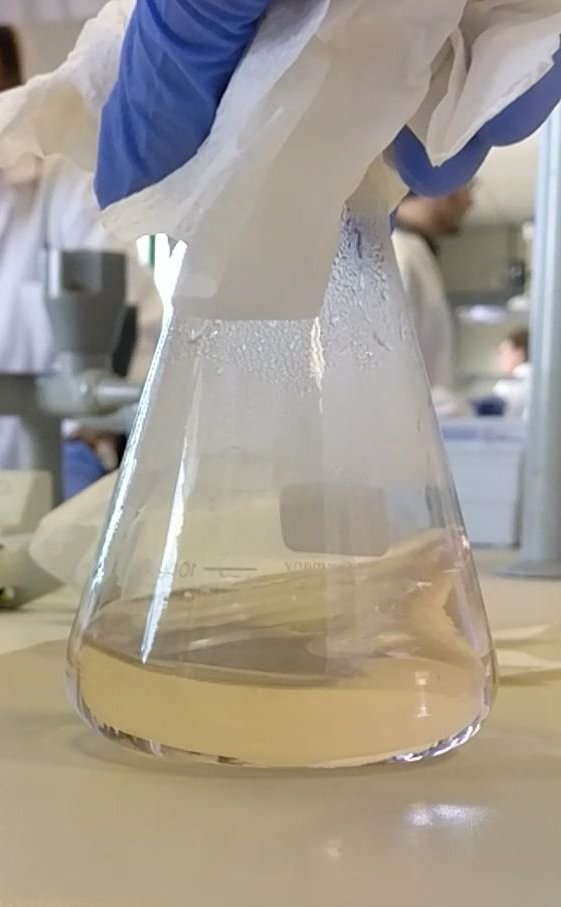
\includegraphics[width=0.3\textwidth]{./immagini/agarosio.jpg}
	% 	\caption{Mescolamento della soluzione con agarosio}
	% 	\label{agarosio}
	%
	% \end{figure}


% \end{enumerate}


\subsection{Risultati e Conclusioni}
